\documentclass{article}
\usepackage{graphicx}
\usepackage{amsmath}
\usepackage{float}
\usepackage{amsfonts}
\usepackage{listings}
\usepackage{xcolor}
\usepackage[utf8]{inputenc}


\lstset{
  language=R,
  basicstyle=\ttfamily\small,
  numbers=left,               % Numérotation des lignes
  numberstyle=\tiny\color{gray}, % Style de la numérotation
  keywordstyle=\color{blue},  % Couleur des mots-clés
  commentstyle=\color{green}, % Couleur des commentaires
  stringstyle=\color{red},    % Couleur des chaînes de caractères
  breaklines=true,            % Coupe les lignes trop longues
  frame=single,               % Encadre le code
}


\title{TP1 ADM}
\author{MARIAC Damien, SCAIA Matteo}
\date{\today} 

\begin{document}

\maketitle

\begin{figure}[h] 
    \centering
    
\includegraphics[width=0.5\textwidth]{ssd_logo.png} 
\end{figure}

\begin{figure}[h] 
    \centering
    
\includegraphics[width=0.5\textwidth]{logo_um_2022_rouge_RVB.png} 
\end{figure}

\newpage

\tableofcontents

\newpage

\section{Introduction}
On dispose d'un jeu de donnees présentant une étude de 27 espèces d'arbres dans 1000 parcelles de la forêt du Congo.
Nous avons enlevé une ligne problématique dans notre jeu de de donnée (ligne 1000 code TGC).
Il s'agit d'étudier la variabilité des densités de peuplement d'espèces arborées dans différentes parcelles de la forêt.
Nous disposons dans notre jeu de donnée de 30 variables quantitatives dont : 27 variables de comptage des espèces, une sur la surface de la parcelle, une forestier et une géologique.
Et d'une variable qualitative "code".
\\
On arrondira les valeurs à $10^{-3}$.

\begin{table}[H]
    \centering
    \begin{tabular}{|l|l|l|l|l|l|l|}
    \hline
    code & gen1 & gen2 & gen3 & forest & geology & surface \\ \hline
    1299 & 0    & 0    & 0    & 2      & 3       & 5       \\ \hline
    2644 & 9    & 0    & 3    & 7      & 6       & 15      \\ \hline
    1838 & 9    & 0    & 0    & 5      & 6       & 17.5    \\ \hline
    534  & 0    & 4    & 0    & 1      & 5       & 20.5    \\ \hline
    3213 & 1    & 1    & 0    & 1      & 6       & 10.5    \\ \hline
    1861 & 19   & 3    & 1    & 7      & 3       & 20      \\ \hline
    \end{tabular}
    \caption{Extrait du jeu de données Datagenus}
\end{table}



\section{Partie 1}
\subsection{inertie et barycentre}

Afin d'avoir une une comparaison plus juste entre chaque parcelles, nous utiliserons la densité de peuplement de ces dernieres. C'est à dire 
la densité de peuplement de chaque espèce d'arbre par unité de surface est donnée par:

\[
\text{d}_i^j = \frac{n_i^j}{S_i}
\]
où \(n_i^j\) est le nombre d'arbres de l'espèce \(j\) présents sur la parcelle \(i\), et \(S_i\) représente la surface de la parcelle \(i\).

\vspace{2\baselineskip}



Nous devons de plus centrer et reduire les variables quantitatives dans le but de mieux comparer celles qui decrivent les différents densité.
Nous allons alors utiliser :
\[
(x_i^j)_{1 \leq j \leq 27} = \frac{x_i^j - \bar{x}^j}{\sigma_j}
\]

Avec $\bar{x}_j$ la moyenne pour la j-eme variable et  $\sigma_j$ l'ecart-type de la j-eme variable.

\vspace{2\baselineskip}

Dans la suite, nous ne considererons plus que les variables centrées-réduites.
De plus, on supposera que le poid de nos parcelles sont equipondérée.
\vspace{2\baselineskip}
\\
\textbf{Par consequents on a:}
\\
\\
\underline{Barycentre à l'origine :} (preuve théorique)
\\

Supposons que nous avons un ensemble de données $X$ composé de $n$ observations et $p$ variables (dans notre cas 1000 et 27). Après le centrage et la réduction, la matrice transformée $X'$ est définie par :

\[
\tilde{x}_{ij} = \frac{x_{ij} - \overline{x}^j}{s_j}
\]

Le barycentre de $X$ est donné par la moyenne de chaque colonne de $X$. Calculons cette moyenne pour n'importe quelle j:

\[
\overline{x}^j = \frac{1}{n} \sum_{i=1}^n \tilde{x}_{i}^j = \frac{1}{n} \sum_{i=1}^n \frac{x_{i}^j - \overline{x}^j}{s_j} = \frac{1}{s_j} \left(\frac{1}{n} \sum_{i=1}^n x_{i}^j\right) - \frac{\overline{x}^j}{s_j} = 0
\]

Ainsi, le barycentre de chaque variable dans $X'$ est zéro.
\\
\\

\underline{Inertie totale égale à 27 :} (preuve théorique)
\\
\\
Considérons la meme matrice de données $\tilde{X}$.


L'inertie de l'ensemble des points $\tilde{X}$ par rapport à leur barycentre $\mathbf{y}$ est définie par:
\[
I_{Y, W} = \sum_{i=1}^n w_i \|\mathbf{\tilde{x}}_i - \mathbf{y}\|^2
\]

Dans notre cas, le barycentre est nulle.
De plus, tous les poids $w_i$ sont égaux (par exemple, $w_i = \frac{1}{n}$ ce qui est notre cas), alors l'inertie devient:
\[
I_{Y, W} = \sum_{i=1}^n w_i \|\mathbf{\tilde{x}}_i\|^2 = \frac{1}{n} \sum_{i=1}^n \|\mathbf{\tilde{x}}_i\|^2 
\]

Comme chaque $\mathbf{\tilde{x}}_i$ est une observation centrée-réduite et la variance de chaque variable est 1, nous avons (pour i fixé):
\[
\|\mathbf{\tilde{x}}_i\|^2 = \sum_{j=1}^p (\tilde{x}_{i}^j)^2 = p
\]

Ainsi, l'inertie totale est:
\[
I_{Y, W} = \frac{1}{n} \sum_{i=1}^n p = p 
\]
Dans notre cas vaut 27.

\subsection{Autour des types forestiers}

Dans cette section, nous calculons les barycentres des sept types forestiers présents dans les données, ainsi que l'inertie inter-types et le coefficient $R^2$ associé à la partition des parcelles selon ces types. Ce calcul nous permet d'évaluer la proportion de la variabilité totale des densités de peuplement.

\subsubsection{Calcul des poids des types forestiers}
Le poids de chaque type forestier est calculé comme la proportion de parcelles appartenant à ce type par rapport à l'ensemble des 1000 parcelles. C'est à dire, le poids est donné par :

\[
p_i = \frac{\text{Nombre de parcelles du type } i}{1000}
\]

\begin{table}[H]
    \center
    \begin{tabular}{|l|l|l|l|l|l|l|}
    \hline
    1     & 2     & 3     & 4     & 5     & 6     & 7     \\ \hline
    0.278 & 0.105 & 0.022 & 0.018 & 0.169 & 0.095 & 0.313 \\ \hline
    \end{tabular}
    \caption{Tabeau des poids forestier}
    \end{table}


\subsubsection{Calcul des barycentres des types forestiers}
Pour chaque type forestier $i$,  (avec $X$ la matrice des densités centrés réduites), le barycentre vaut :

\[
\bar{X}_i = \frac{1}{n_i} \sum_{j \in \text{Type } i} X^j
\]

Avec $n_i$ le nombre de parcelles dans le type forestier i.
\\
Nous obtenons alors une matrice $B \in \mathcal{M}_{7,27}(\mathbb{R})$


\subsubsection{Calcul des normes euclidiennes carrées}
Une fois les barycentres calculés, nous évaluons la distance de chaque barycentre à l'origine:

\begin{table}[H]
    \begin{tabular}{|l|l|l|l|l|l|l|l|}
    \hline
    type forestier       & 1         & 2         & 3         & 4      & 5     & 6     & 7     \\ \hline
    distance (en norme 2) & 0.772 & 3.228 & 4.279 & 21.210 & 1.092 & 1.443 & 1.628 \\ \hline
    \end{tabular}
    \caption{normes carrée}
    \end{table}

\subsubsection{Inertie inter-types et coefficient $R^2$}


L'inertie inter-types forestiers est calculée en pondérant les normes euclidiennes carrées par les poids des types forestiers. Elle mesure la variabilité des densités de peuplement expliquée par la partition en types forestiers et elle est définie par :

\[
\text{Inertie inter-types} = \sum_{i=1}^{7} p_i \|\bar{X}_i\|^2 = 1.860
\]

Le coefficient $R^2$ nous permet d'évaluer dans quelle mesure les types forestiers expliquent la variabilité des densités de peuplement dans les parcelles observées.
\[
R^2 = \frac{\text{Inertie inter-types}}{\text{Inertie totale}}=0.069
\]

Cela correspond à une disparité d'environ 7\%

\subsection{Liaisons}

On s'interesse maintenant à l'interpretation des resultats trouvé. Nous calculons alors le $R^2$ de chaque variable densité avec
 $R^2 = \frac{variance_{inter -typesforestiers}}{variance totale}$.

\begin{table}[H]
    \centering
    \begin{tabular}{|l|l|l|l|l|}
    \hline
    Especes & gen1  & gen6  & gen17 & gen25 \\ \hline
    R²      & 0.072 & 0.008 & 0.096 & 0.184 \\ \hline
    \end{tabular}
    \centering
    \caption{Extrait du R² des variables}
    \end{table}


Nous remarquons numériquement que la variable la plus lié au type est gen25, tandis que la moins lié est gen6.

Montrons que le $R^2$ de la partition est la moyenne (arithmétique) des $R^2$ des densités:

\[
R^2 = \frac{\text{Inertie externe}}{\text{Inertie totale}}
= \frac{1}{27} \sum_{k=1}^{7} \lVert x_k^j \rVert^2
= \frac{1}{27} \sum_{k=1}^{7} \sum_{j=1}^{27} (x_k^j)^2
= \frac{1}{27} \sum_{j=1}^{27} \sum_{k=1}^{7} (x_k^j)^2
= \frac{1}{27} \sum_{j=1}^{27} R_j^2
\]

On retrouve bien numériquement la même valeur :
\\
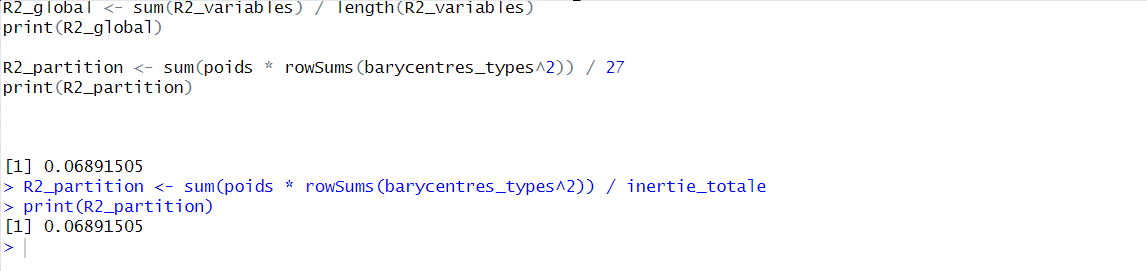
\includegraphics[width=1.5\textwidth]{preuve_info_p1.png}

\newpage
\section{Partie 2}
\subsection{Enoncer}
On notera $X$ la matrice dont les colonnes sont les 27 densités centrées-réduites, $Y$ la
matrice dont les colonnes sont les indicatrices de types forestiers, et $Z$ celle dont les
colonnes sont les indicatrices de sols (geology). \\
On notera $W=\frac{1}{n}I_n$ la matrice des poids des individus et $M=\frac{1}{p}I_p$
celle des poids des variables.
\subsection{Rappel et calcul de projecteur}
\subsubsection{Rappel}
Montrons l'égalité suivante. \\
\[
\forall j \hspace{0.5cm} \Pi_Y x^j = \Pi_{Y^c} x^j
\]
Tout d'abord, il est important de rappeler que les $x^j$ sont des variables qui sont
centrées réduites. De plus, nous rappelons que 
\[
Y^c = \Pi_{1^\perp} Y 
\]
\[
\Pi_Y = \Pi_{Y^c} + \Pi_1
\]
A partir de ces deux résultats, nous pouvons conclure que. \\
\begin{align*}
    \Pi_Y x^j & = \Pi_{Y^c} x^j + \Pi_1 x^j \\
    &= \Pi_{Y^c} x^j
\end{align*}
Nous venons de montrer que pour tout $j$, 
\[
\Pi_Y x^j = \Pi_{Y^c} x^j
\]
De plus, nous fixons $j$, et nous avons l'expression suivante.
\[
\left\lVert \Pi_Y x^j \right\rVert^2 _W = \left\langle \Pi_Y x^j,\Pi_Y x^j\right\rangle_W
\]
Or, il est important de préciser que
\[
\Pi_Y x^j=\sum_{q = 1}^{p}\Pi_{y^q} x^j=\sum_{q = 1}^{p}y^q( \overline{x^j}^q - {\overline{x^j}} )  
\]
Ici, $\overline{x^j}$ représente la moyenne globale des $x^j$, $\overline{x^j}^q$ représente la moyenne pondérée des $x^j$ pour le type forestier $q$.\\
A partir de ces notations, nous avons l'expression suivante.
\begin{align*}
    \left\lVert \Pi_Y x^j \right\rVert^2 _W &= \left\langle \Pi_Y x^j,\Pi_Y x^j\right\rangle_W \\
     &=  \sum_{q = 1}^{p}( \overline{x^j}^q - {\overline{x^j}} ) \sum_{ i= 1}^{p}( \overline{x^j}^i - {\overline{x^j}} )\left\langle y^q,y^i\right\rangle_W \\
     &= \sum_{q = 1}^{p}w^q( \overline{x^j}^q - {\overline{x^j}} )^2
\end{align*}
Nous pouvons conclure que $\left\lVert \Pi_Y x^j \right\rVert^2 _W$ s'interprete statistiquement comme
étant la mesure des variation des $x^j$ dans un certain type forestier.
\\
\\
\subsubsection{Calcul de projecteur}
Le but de cette question est de trouver l'expression
de $\Pi_Y$ et de calculer pour tout $j \in [1,27]$, $\Pi_{x^{j}}$ et $tr(\Pi_{x^{j}}\Pi_Y)$. Nous ferons la démonstration
puis nous programmerons le résultat. \\
Tout d'abord, on admet l'expression suivante.
\[
\Pi_Y = Y(Y'WY)^{-1}Y'W
\]
Soit $j \in [1,27]$. Calculons les deux expressions donné précédemment.
\[
\Pi_{x^j}= x^{j}(x^{j\prime}Wx^{j})^{-1}x^{j\prime}W
\]
En utilisant les propriétés de la trace et l'expression de $\Pi_{x^j}$, il suit que 
\begin{align*}
    tr(\Pi_{x^{j}}\Pi_Y) &= tr(x^{j}(x^{j\prime}Wx^{j})^{-1}x^{j\prime}W\Pi_Y) \\
    &=tr((x^{j\prime}Wx^{j})^{-1}x^{j\prime}W\Pi_Yx^{j})\\
    &=(x^{j\prime}Wx^{j})^{-1}x^{j\prime}W\Pi_Yx^{j}\\
    &= \frac{\left\langle x^{j\prime},\Pi_Yx^{j}\right\rangle_W }{\left\lVert x^j\right\rVert^2_W }\\
    &= R^2(x^j\mid Y )
\end{align*}
Donc, nous pouvons conclure que $tr(\Pi_{x^{j}}\Pi_Y)$ 


\newpage
\section{Conclusion}

\newpage
\lstinputlisting{C:/Users/damie/Desktop/MASTER/ADM/tp/tp1/tex/TP1.R}

\end{document}
